\documentclass[11pt]{article}
\input{/Users/markwang/.preamble}
\begin{document}

\subsection*{Decision Problems}

\begin{center}
    Why formulate problems as decision problems ?
\end{center}
\begin{enumerate}
    \item Decision problems are in essence easier than the corresponding optimization problems. So by proving the decision problem is hard, the optimization problem must be as least as hard 
    \item In many cases, both the decision problem and its corresponding optimization problem are equivalent
\end{enumerate}

\[
    \mathcal{P} = \{ \text{ Problems that can be solved in polynomial time } \}
\]
\[
    \mathcal{NP} = \{ \text{ Problems that can be verified in polynomial time } \}
\]

\begin{proposition*} \textbf{Naive algorithm for $\mathcal{NP}$ problems} \\
    All problems in $\mathcal{NP}$ can be solved by a \textbf{generate-and-verify} algorithm with the following structure 

    \begin{algorithm}[H]
        \SetKwFunction{verify}{Verify}
        \SetKwFunction{gv}{Generate-and-Verify}
        \SetKwFunction{true}{True}
        \SetKwFunction{false}{False}

        \Fn{$\gv(x)$}{
            \text{Generate all certificates}
            \For{\text{each } $c\in $ certificates}{
                \If{\verify$(x,c)$}{
                    \Return{\true}
                }
            }
            \Return{\false}
        }        
    \end{algorithm}
\end{proposition*}


\begin{example} \textbf{Composite} \\ 
    Given positive integer $x$, does $x$ have any factor (i.e. a composite number)

    \begin{algorithm}[H]
        \SetKwFunction{verify}{Verify}
        \SetKwFunction{comp}{Composite}
        \SetKwFunction{true}{True}
        \SetKwFunction{false}{False}

        \Fn{$\comp(x)$}{
            \text{Generate all certificates}
            \For{for all integer $c\in 2$ \KwTo $x-1$}{
                \If{$c$ divides $x$}{
                    \Return{\true}
                }
            }
            \Return{\false}
        }        
    \end{algorithm}
\end{example}

\begin{defn*}
    $B$ is an efficient \textbf{certifier} for a problem $X$, if the following properties hold:
    \begin{enumerate}
        \item $B$ is a polynomial time algorithm that takes two input $s$, the input, and $t$, the certificate and returns either $yes$ or $no$ to the problem $X$
        \item There is a polynomial time function $p$ such that for every string $s = \{ 0, 1\}*$, we have $s\in X$, i.e. $s$ is a $yes$ solution to $X$, if and only if there exists a string $t$ such that $|t| \leq p(|s|)$ (i.e. $|t| \leq |s|^2$ say) and $B(s,t)$ is $yes$ (implies the loop is not over infinite number of times, i.e. there is an upper bound on the loop)
    \end{enumerate}
    $s\in X$ means $s$ is an $yes$ instance of $X$
\end{defn*}


\begin{theorem*}
    \[
        \mathcal{P} \subseteq \mathcal{NP}
    \]
    \begin{proof}
        Consider a decision problem $X\in \mathcal{P}$. This implies there exists a polynomial time algorithm $A$ that solves $X$. To show $X\in \mathcal{NP}$, we want to find an efficient verifier $B(s,t)$ for $X$, such that $B(s,t) = A(s)$ for any $t$. Dont know...
    \end{proof}
\end{theorem*}

\begin{defn*}
    A problem $X$ is called $\mathcal{NP}$-complete (NPC) if 
    \begin{enumerate}
        \item $x\in \mathcal{NP}$
        \item $\mathcal{NP}$-hard, i.e. for every $Y\in \mathcal{NP}$, $Y\leq_p X$
    \end{enumerate}
\end{defn*}

\begin{example}
    \textbf{Prove NP}\\

    \begin{enumerate}
        \item $\textsc{Independent Set} \in \mathcal{NP}$. For the set $S = \{v_1,\cdots, v_n \}$ The verification steps takes every $v_i \in S$ and check $G.Adj[v_i]$ (totals to $|E|$) takes $k(|V| + |E|)$ steps at most. But $k\leq |V|$ so takes $|V|(|E| + |V|)$
        \item 
    \end{enumerate}
    
\end{example}


\begin{defn*}
    $X$ in $\mathcal{NP}$ means there is a certifier $B(s,t)$ running in polynomial time such that 
    \[
        B(s,t) = 
        \begin{cases}
            true & \text{ for some $t$ where $s$ is a $yes$ instance of $X$} \\
            false & \text{ for all $t$ where $s$ is a $no$ instance of $X$} \\ 
        \end{cases}
    \]
    $co\mathcal{NP}$ is the complement of problems in $\mathcal{NP}$, i.e. problems whose no-instances are easy to verify 
    \[
        B(s,t) = 
        \begin{cases}
            true & \text{ for all $t$ where $s$ is a $yes$ instance of $X$} \\
            false & \text{ for some $t$ where $s$ is a $no$ instance of $X$} \\ 
        \end{cases}
    \]
\end{defn*}

\begin{example}
    \textbf{Examples of $co\mathcal{NP}$ algorithms}
    \begin{enumerate}
        \item \textbf{Prime}
            \begin{algorithm}[H]
            \SetKwFunction{prime}{Prime}
            \SetKwFunction{true}{True}
            \SetKwFunction{false}{False}

            \Fn{$\prime \in co\mathcal{NP}$}{
                For input $x$ \\
                \For{$c = 2, \cdots, x-1$}{
                    \If{$c$ divides $x$}{
                        \Return{\false}
                    }
                }
                \Return{\true}
            }
        \end{algorithm}
        \item \textbf{Dense set} $\in co\mathcal{NP}$
    \end{enumerate}
\end{example}

\begin{proposition*}
    \[
        \mathcal{P} \subseteq co\mathcal{NP}
    \]
\end{proposition*}



\subsection*{NP-completeness problems are hardest problems in NP}


\begin{example}
    \textbf{SAT} (Satisfiability problems)
    \begin{enumerate}
        \item \textbf{Circuit-SAT} Given a circuit with AND, OR, NOT gates and input set $I$ and a single output $x$. The question asks if there is a set of $I$ such that $x = T$ (satisfiability) If the answer is $yet$, the circuit is \textbf{satisfiable} otherwise \textbf{unsatisfiable}. 
        \item \textbf{SAT} Since any circuit can be transformed into a boolean expression, is an equivalent question for such boolean formula, i.e. if the value of formula yields $true$ or $false$
        \item \textbf{CNF-SAT} Conjunctive normal form. 
        \[
            \phi = c_1 \land \cdots c_i  \cdots \land c_k  \quad \quad c_i = (t_{i_1} \lor \cdots \lor t_{i_j})
        \]
        where $t_{i_j} = x_j$ or $\neg x_j$. Note every boolean expression can be converted to CNF
        \item \textbf{3-SAT} A special form of CNF-SAT where each clause  $c_i$ has exactly 3 literals. Again can convert from every CNF.
    \end{enumerate}
\end{example}

\begin{theorem*}
    SAT is NPC. Given a boolean formula $\phi$, ask the question if $\phi$ is satisfisable. Let $X$ be SAT-family of problems
    \begin{proof}
        Prove by definition of NPC (2-part)
        \begin{enumerate}
            \item Prove $X\in \mathcal{NP}$. Given $\phi$ where $t$ is the truth assignment of the variables in $\phi$. Given $t$, verify $\phi$ is true is easy, since can just substitute variable in and evaluate using boolean expression. Hence can be verified easily
            \item Prove $Y\leq_q X$ for all $Y\in NP$. Basic idea, every NP problem can be reduced to circuits (Circuit-SAT). 
        \end{enumerate}
    \end{proof}
\end{theorem*}

\begin{example}
    Given a graph $G = (V,E)$ Does it contain a 2 node independent set. 
    \begin{solution}
        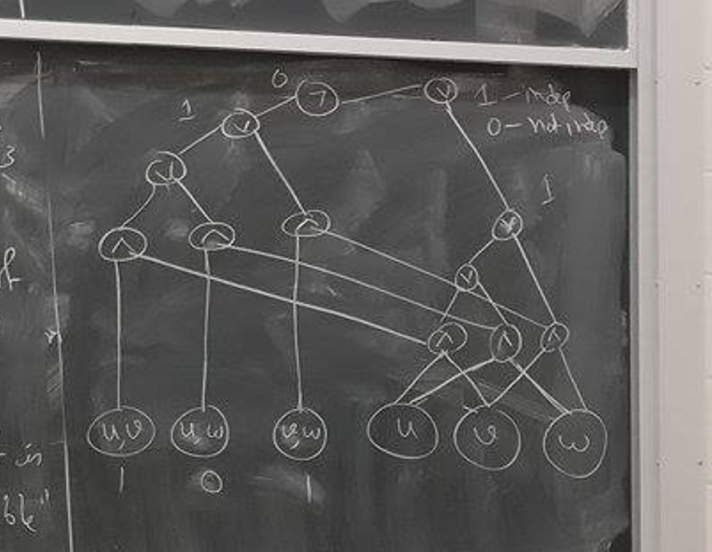
\includegraphics[width=\textwidth/2]{circuit_1}
    \end{solution}
\end{example}

\begin{defn*}
    \textbf{Techniques for prooving NPC} \\
    To prove $X$ is NP-hard, use a known NP-hard problem $Y$ and show that $Y\leq_q X$
    \begin{proof}
        Note If $A\leq_p B$ and $B\leq_p C$ then $A\leq_q C$. So if $Y$ is NP-hard, then $\forall Z\in \mathcal{NP}$, $Z \leq_p Y$. And since $Y\leq_p X$, so $\forall Z\in \mathcal{NP}$, $Z\leq_p X$, so $X$ is NP-hard
    \end{proof}
\end{defn*}

\begin{proposition*}
    \textbf{3-SAT} is NPC 
    \begin{proof}
        Idea: Reduce it to $SAT$, which was shown to be NP-hard
        \begin{enumerate}
            \item 3-SAT $\in NP$, true...
            \item Now we prove $CNF-SAT \leq_p 3-SAT$. Given a formula $\phi$ in CNF, obtain an formula $\phi'$ in 3-SAT, such that $\phi$ is satisfiable if and only if $\phi'$ is satisfiable. Let $\phi = c_1 \land \cdots \land c_r$ where $c_i = (x_{j_i} \lor \cdots \lor x_{j_k})$ Want to size of each $c_i$ to 3. For each $c_i$ in $\phi$, if 
            \begin{enumerate}
                \item If $c= (a_1)$ then replace $c$ with $(a_1 \lor a_1 \lor a_1)$.
                \item If $c = (a_1 \lor a_2)$, then replace $c$ with  $(a_1 \lor a_1 \lor a_2)$. 
                \item If $c =  (a_1 \lor a_2 \lor a_3)$, then leave it as is. 
                \item If $c = (a_1 \lor a_2 \lor \cdots \lor a_s)$ where $s>3$, then replace $c$ with $c' = (a_1 \lor a_2 \lor a_3) \land (\neg z_1 \lor a_3 \lor z_2) \land (\neg z_2 \lor a_4 \lor z_3) \land \cdots \land (\neg z_{s-4} \lor a_{s-2} \lor z_{s-3}) \land (\neg z_{s-3}\lor a_{s-1} \lor a_{s})$  where $(z_1,\cdots, z_{s-3})$ are new variables. Now we prove $c$ is satisfiable if and only if $c'$ is satisfiable 
                
                \begin{enumerate}
                    \item ($=>$) There is a truth assignment $a_1,\cdots a_s$ that makes $c$ true. This implies that there is some $a_i = T$ the first $i$ such that $a_i = T$.
                    \begin{enumerate}
                        \item  If $i = 1$ or $2$, let $z_1,\cdots, z_{s-3} = F$, then every clause is true. 
                        \item If $i = s-1$ or $s$, let $z_1,\cdots, z_{s-3} = T$, then every clause is true 
                        \item If $2<i<s-1$, let $z_1,\cdots, z_{i-2} = T$ and let $z_{i-1},\cdots, z_{s-3} = F$, then every clause is true  
                    \end{enumerate}
                    \item ($<=$) If there is a truth assignment that makes $c'$ true, we want to show that there is a truth assignment that makes $c$ is true. Obvious, the same assignment works
                \end{enumerate}

            \end{enumerate}
            
            
           
        \end{enumerate}
    \end{proof}
\end{proposition*}


\end{document}
